\section{Zwiększenie wpływu hubów, zmiana rozkładu}

Huby powinny mieć większy dar przekonywania. W celu uzyskania takiego efektu należało zwiększyć siłę oddziaływania węzłów z dużą liczbą sąsiadów.
W związku z tym średnia opinii sąsiadów została zmieniona na średnią ważoną, gdzie wartościami wag będą współczynniki wpływu $A_i$ każdego z nich.
Spowoduje to zawężenie przedziału rozkładu, z którego jest losowana nowa wartość opinii.
W związku z tą zmianą nowe wyniki symulacji wyglądają następująco:
\begin{table}[htbp]
    \centering
    \begin{tabular}{c|c|c|c}
        \hline
        Populacja & \multicolumn{3}{c}{Średnia liczba iteracji}                                    \\
        \hline
                  & Erdős-Rényi                                 & Barabási-Albert & Watts-Strogatz \\
        \hline
        20        & 6,4                                         & 8,4             & 10,2           \\
        50        & 5,4                                         & 12,4            & 14,7           \\
        100       & 6,3                                         & 13,9            & 17,8           \\
        200       & 6,4                                         & 16,1            & 22,0           \\
        500       & 7,1                                         & 20,2            & 29,3           \\
        1000      & 8,0                                         & 21,1            & 35,7           \\
        2000      & 8,3                                         & 29,3            & 34,9           \\
        5000      & 8,3                                         & 14,7            & 41,9           \\
    \end{tabular}
    \caption{Wyniki symulacji ze średnią udziału sąsiadów agenta w populacji i średniej opinii sąsiadów}
    \label{tab:results_with_neighbour_opinion_weighted_average}
\end{table}

Jak widać w tabeli \ref{tab:results_with_neighbour_opinion_weighted_average}, wyniki zmieniły się znacząco tylko dla sieci Watts-Strogatz,
pozostałe sieci zbiegały mniej więcej tak samo szybko.

W związku z tym sposobem na spowolnienie zbiegania opinii do jednego punktu stała się zmiana rozkładu.
Wybór padł na rozkład wykładniczy.

\begin{figure}
    \centering
    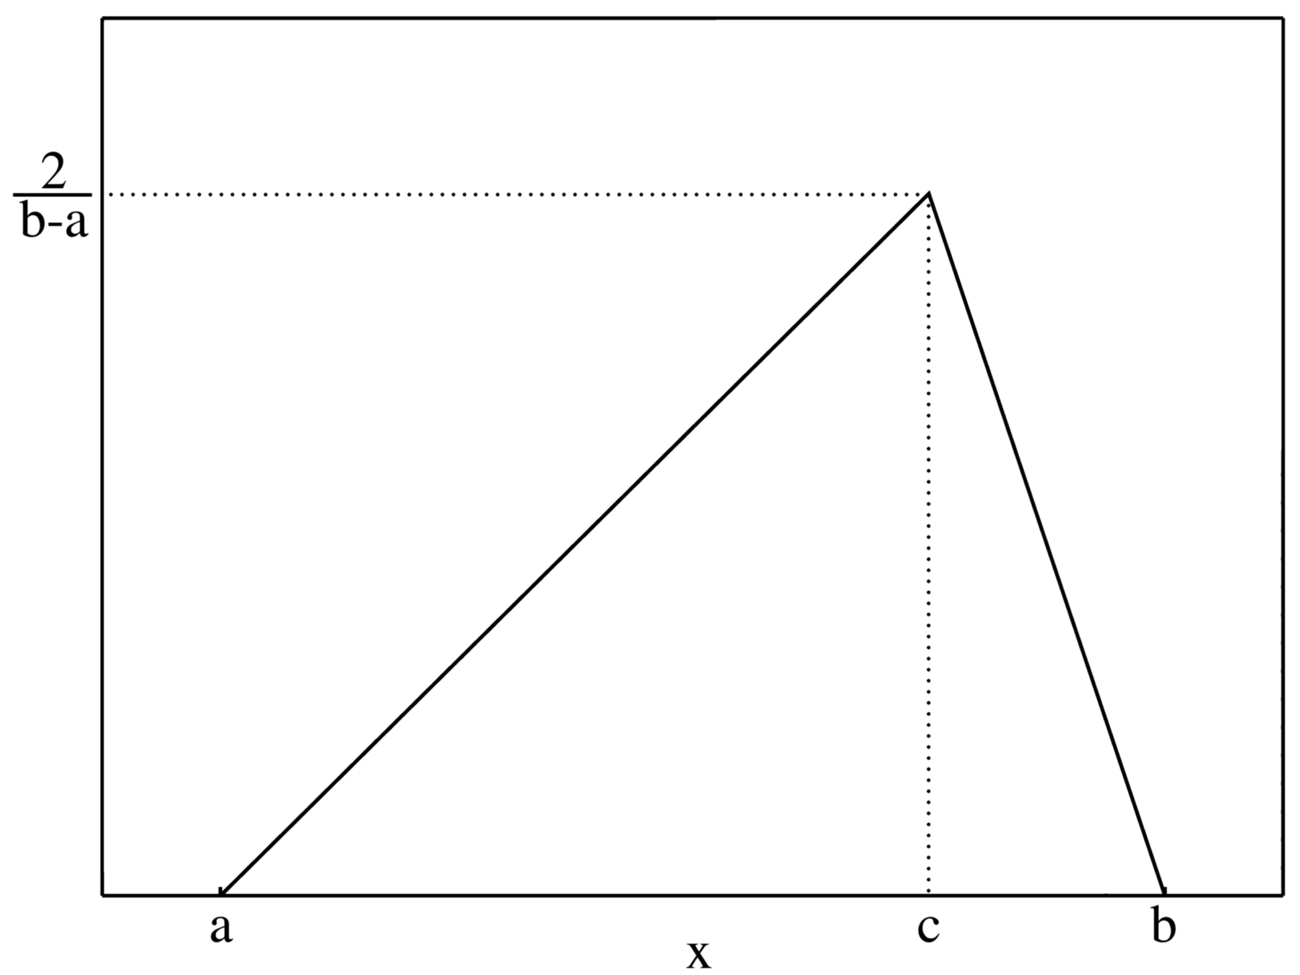
\includegraphics[width=0.5\textwidth]{img/Triangular_distribution_PMF.png}
    \caption{Rozkład trójkątny. Źródło: \cite{rozklad_trojkatny_wykres}}
    \label{fig:rozklad_trojkatny}
\end{figure}
\begin{figure}
    \centering
    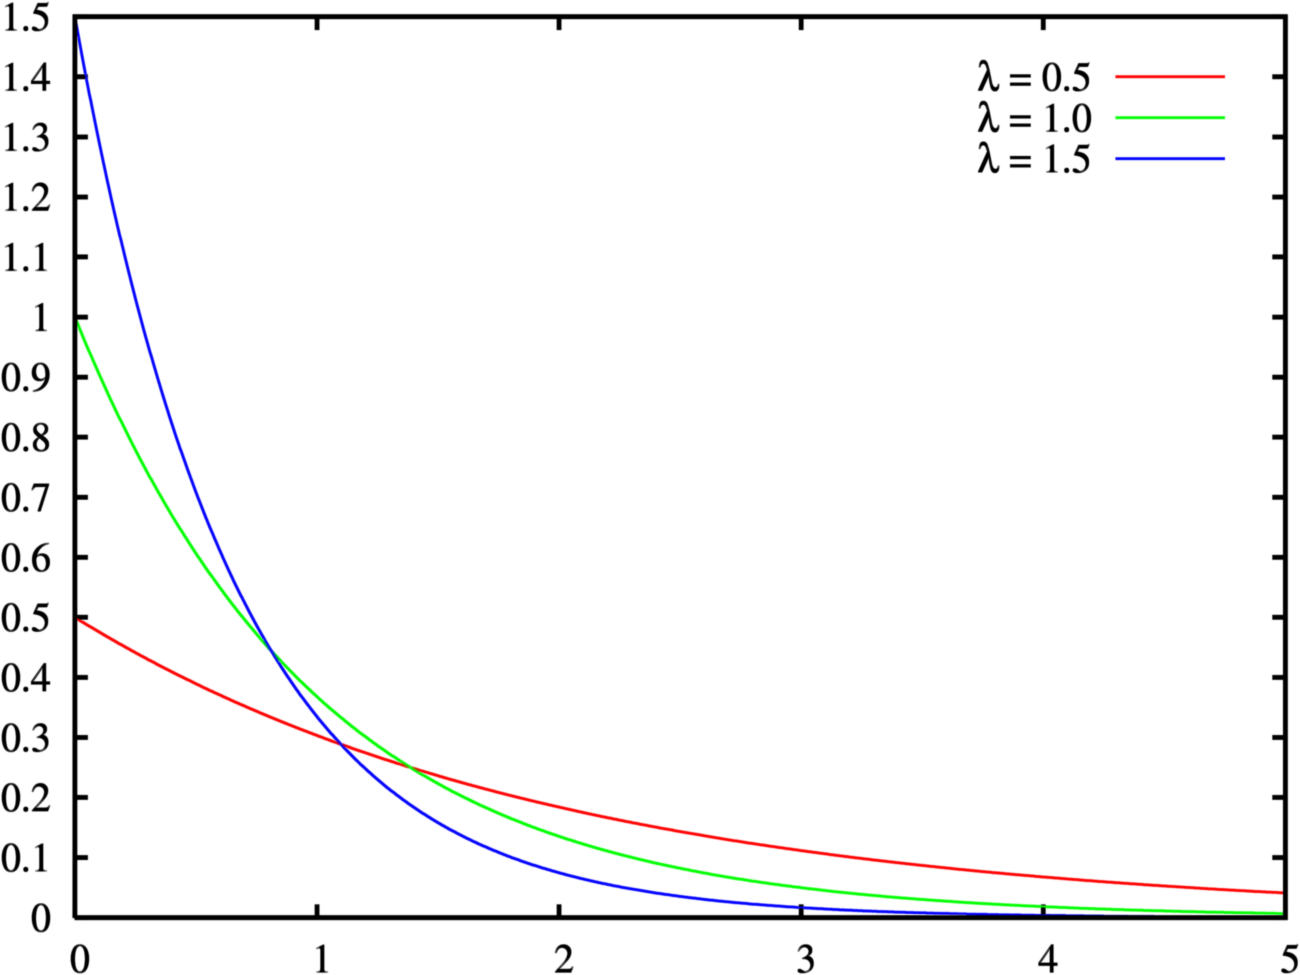
\includegraphics[width=0.5\textwidth]{img/Exponential_distribution_pdf.png}
    \caption{Rozkład wykładniczy. Źródło: \cite{rozklad_wykladniczy_wykres}}
    \label{fig:rozklad_wykladniczy}
\end{figure}

Rezultat zmiany rozkładu prezentowany jest w tabeli \ref{tab:results_with_exponential_distribution}.

\begin{table}[htbp]
    \centering
    \begin{tabular}{c|c|c|c}
        \hline
        Populacja & \multicolumn{3}{c}{Średnia liczba iteracji}                                    \\
        \hline
                  & Erdős-Rényi                                 & Barabási-Albert & Watts-Strogatz \\
        \hline
        20        & 1420,6                                      & 1384,1          & 1526,6         \\
    \end{tabular}
    \caption{Wyniki symulacji ze średnią udziału sąsiadów agenta w populacji i średniej opinii sąsiadów}
    \label{tab:results_with_exponential_distribution}
\end{table}

Jak widać w tabeli \ref{tab:results_with_exponential_distribution}, przy użyciu rozkładu wykładniczego wyniki symulacji zmieniły się znacząco.
Okazało się, że zaszła potrzeba ograniczenia populacji agentów, ponieważ opinie agentów przestały zbiegać w szybkim tempie.
Oznacza to, że w tej postaci symulacji można będzie zaobserwować, jak kształtują się opinie agentów, i czy dochodzi do polaryzacji poglądów,
tzn. skupienia się opinii w co najmniej dwóch hubach.